\chapter{算法整合与数据挖掘平台实现}

本章将在上一章节提出的短文本数据流集成分类算法的基础上,设计一个用户友好、逻辑清晰、运行高
效的面向社交网络数据的Web数据挖掘
平台。该平台基于Django 网络应用程序开发框架,整合数据挖掘算法,提供可视化的前端界面。在该
平台的设计中,使用了较为流行的MVC开发模式,使得前后端分离,这样组织的代码结构清晰,易于后
期维护
和功能拓展,提高代码运行效率。

\section{面向社交网络的数据挖掘平台设计}

在对“面向社交网络的数据挖掘平台设计”的软件进行设计时,需按照软件工程的开发流程完成。软件设计包括对软
件进行需求分析、功能设计、架构设计、API设计和服务器部署设计。软件设计是开发中的最重要一环,
也是优秀开发者必须进行的工作。“面向社交网络的数据挖掘平台设计”解决的是“怎样做”的问题。开发
的软件系统满足可用性和稳定性要求,还需对后续扩展维护提供便利。

\subsection{系统设计目标}
本系统核心算法使用SVM作为基分类器,将数据流进行分块,并考虑到对概念漂移的检测,构建高效可
用的集成学
习模型。本文事先使用Twitter API抓取推文数据,对算法进行测试,测试结果表明该算法具有良好的
拟合能力,能够对文本主题实时分类和追踪。接着,在此算法的基础之上,本文构建了一个的可视化的数据挖掘平台,将文本挖掘的一般步骤UI化,使其能更
好与用户进行交互,达到功能可复用、可交互的目的。
本系统的技术栈是Python+Scikit-Learn+Django+MongoDB ,它集成了数据上传、数据预处理与清洗、数据建模、数据可视
化等常用的数据挖掘技术,使得用户无需了解算法和数据挖掘技术内部的运行机制,即可完成对数据的
分析工作。同时,该系统考虑到扩展性问题,当新的数据挖掘算法被提出时,也可以很方便地进行整合。

\subsection{系统架构设计}
根据本系统的设计目标,将其划分4个模块,分别是数据上传、数据预处理、主题跟踪和数据可视化。
图\ref{fig:platform}是本系统的整体架构图:

\begin{figure}
  \centering
  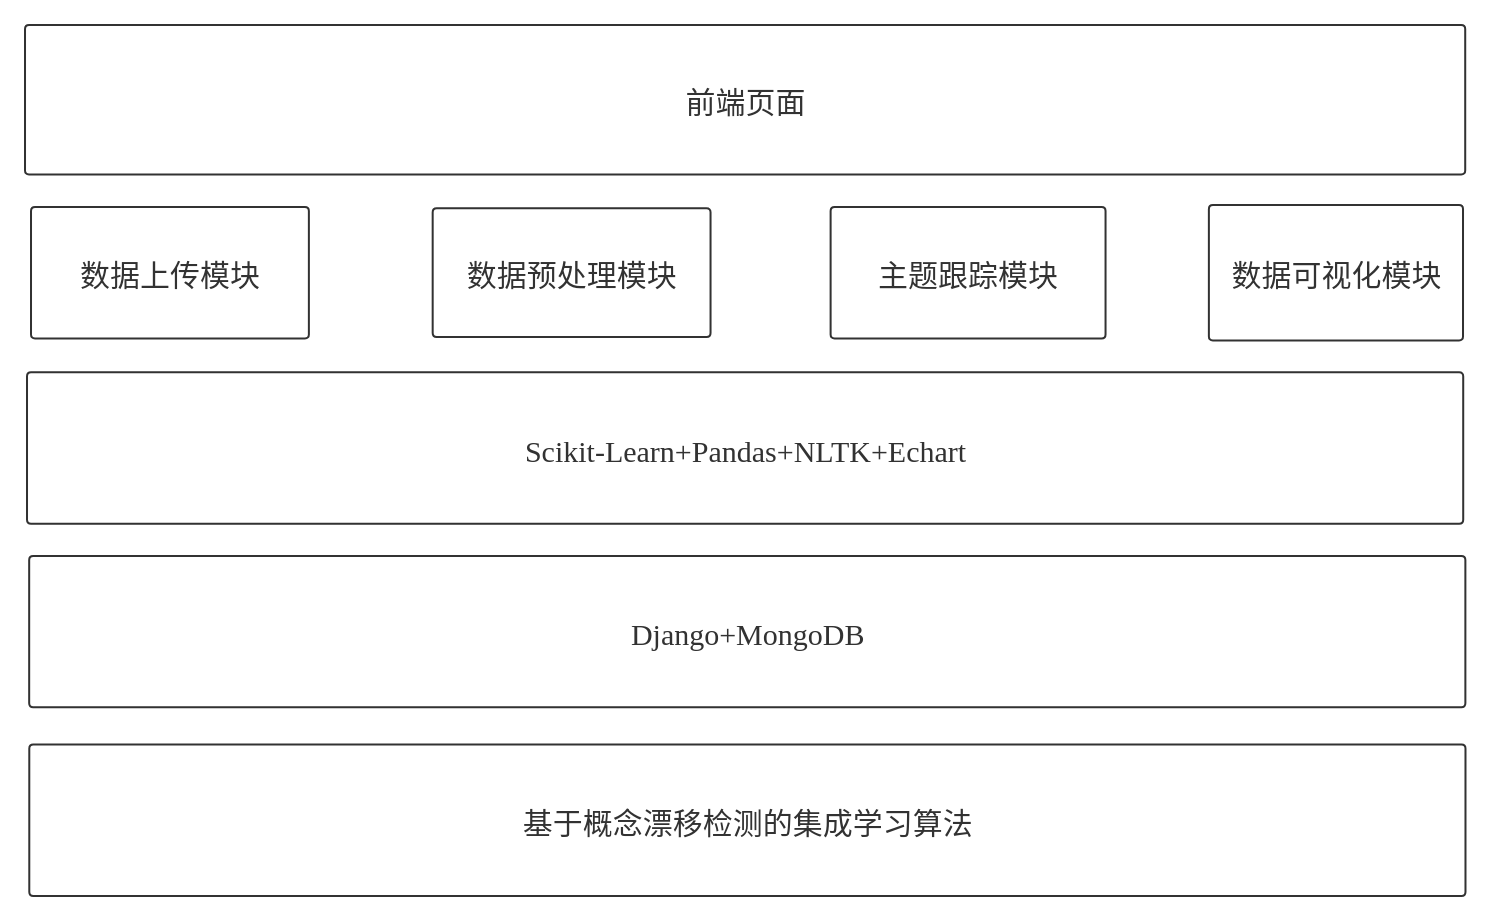
\includegraphics[width=1.0\textwidth]{platform}
  \caption{数据挖掘可视化平台架构图}
  \label{fig:platform}
\end{figure}

本文采用MongoDB作为数据库,由于着重于算法研究,本文数据库较为简单,只有数据内容、数据标签
和时间等项。

\subsection{系统功能模块}
系统的功能模块主要包含四个部分,分别是:数据上传模块、数据预处理模块、主题跟踪模块和数据可
视化模块。各个模块的主要功能如下:
\begin{description}
\item [数据上传:]用于将本地的数据文件导入到MongoDB中;
\item [数据预处理:]负责对上传后的文档进行去停用词、词干提取、词形转换、去噪等操作;
\item [主题跟踪:]本平台的核心模块,是集成学习的算法整合;
\item [数据可视化:]对数据和主题跟踪结果进行了图表展示;
\end{description}

\section{系统实现}

\subsection{软硬件环境}
本次实验的所有模型框架均在python3.6上运行,为保证代码运行稳定、高效,基于Scikit-Learn机器
学习框架进行二次开发,它的特点是可以快速实现研究人员的想法而不拘泥于模型细节。平台运行环境
分本地环境和服务器端环境。本地用于算法的实现与测试,服务器端用于部署整合算法的Django服务。

\begin{table}[H]
  \begin{singlespace}
    \renewcommand{\arraystretch}{1.5} %控制行高
    \centering\caption{软硬件环境}\label{tab:env}                              
    \begin{tabular}{cl}\hline
      环境 & 硬件信息 \\ \hline                                                
      \verb|本地环境| & 操作系统: Debian 10 Testing 版 \\
           & CPU:Intel Core i5 5300U 2.3GHz \\
           & RAM:8.00GB \\
           & 显卡:Intel(R)HD Graphics 630(1024MB)  \\      
           & 硬盘:NVMe SAMSUNG MZVLW128(128GB)+1T机械硬盘 \\ \hline
      \verb|服务器环境(阿里云计算平台)| & 操作系统: Debian 9 Stable版 \\
           & CPU:1.0GHz \\
           & RAM:2.00GB \\
           & 带宽:2M \\ \hline
    \end{tabular}                                                              
  \end{singlespace}                                                            \end{table}               

% \subsection{实验数据集}
% 本文数据通过借助Twitter官方提供的“关键字”API进行采集。一共爬取了从2011年11月到2013年1月的
% 5个类别的共约6万条数据。

\subsection{数据上传模块}
数据上传模块主要用于上传本地文件到数据库中,用户通过在前端页面点击“文件路径”按钮,即触发文
件上传控件,用户通过弹出的文件目录浏览功能访问本地文件,选中后既可获得文件路径,并会自动填
充文件名到“数据集标签”中。

本地文件格式为\texttt{.csv},文件名即为类标签,文件的每一行代表一条推文数据,每一列为该推文的属性,其中包括发布人TwitterID、是否转推、发布时间、推文内容等。由于本文并不需要所有属性,数据上传时就需先对需要的文本进行提取,保留发布人时间、正文内容以及类标签。图\ref{fig:upload}是数据上传模块参数设置。

\begin{figure}[htb]
  \centering
  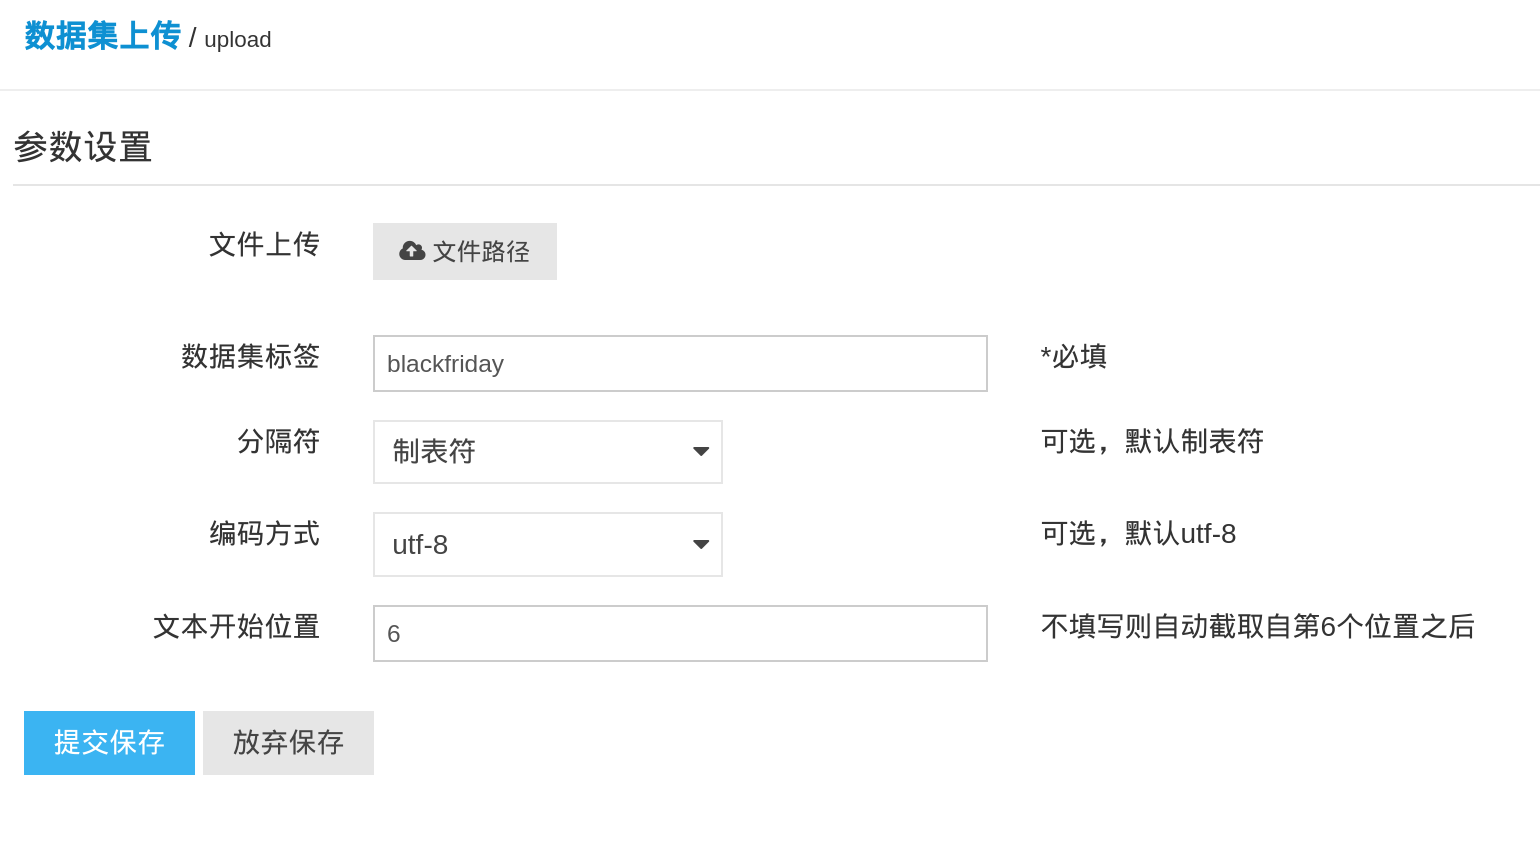
\includegraphics[width=0.8\textwidth]{upload}
  \caption{数据上传参数设置}
  \label{fig:upload}
\end{figure}

设置好其他参数分割符、编码方式、文本开始位置等后,点击提交保存,前端Javascript就会发起ajax请求,django接受到请求后,url机制会匹配到对于视图模块,调用相应的方法,对数据进行保存。

\begin{minted}{py}
urlpatterns = [
    re_path(r'^$', upload),
    re_path(r'uploadfile', upload_file)
]
\end{minted}


\begin{figure}[H]
  \centering
  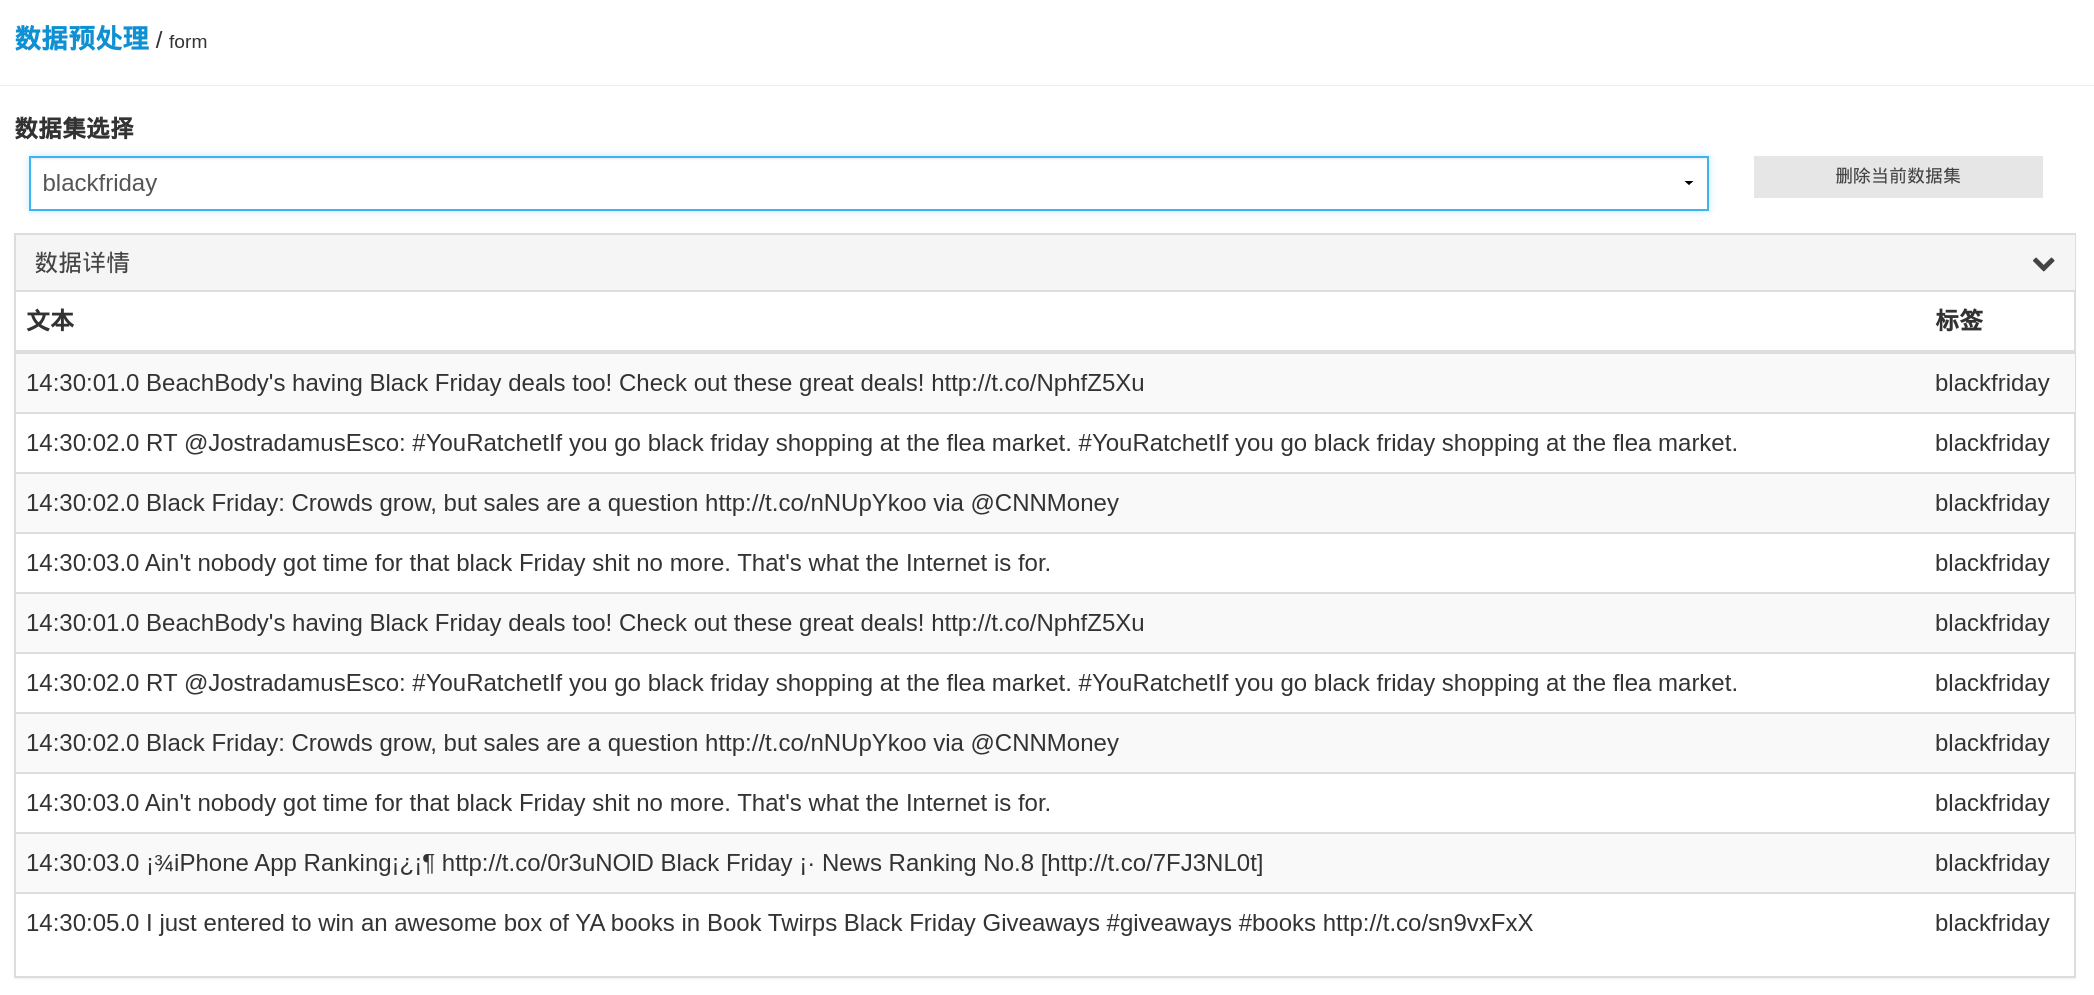
\includegraphics[width=0.8\textwidth]{upload_data}
  \caption{上传数据展示}
  \label{fig:upload_data}
\end{figure}

图\ref{fig:upload_data}是上传后的数据集blackfriday。

\par\subsection{数据预处理模块}
数据预处理模块用于负责对上传后的文档进行去停用词、词干提取、词形转换、去噪等操作。用户在前
端页面选好需要处理的一类文档,选择停用词词库,询问是否进行词干提取、词形转换、大小写转换,
自定义正则表达式等。图\ref{fig:preprocessing}为数据预处理模块的参数设置。

\begin{figure}[H]
  \centering
  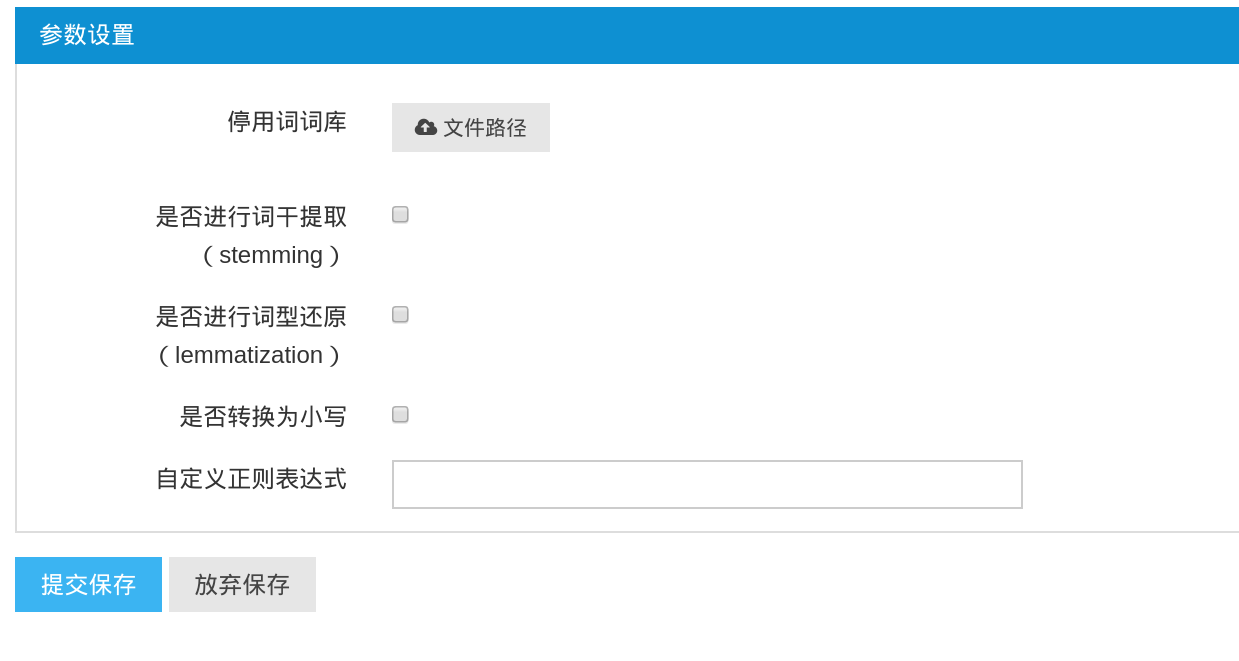
\includegraphics[width=0.8\textwidth]{preprocessing}
  \caption{数据预处理参数设置}
  \label{fig:preprocessing}
\end{figure}

用户点击“提交保存”后,前端Javascript发起ajax POST请求,url路由匹配到相应的视图并进行函数调
用,对选中的文本数据集进行数据预处理。通过ORM条件查询获得表单对象,遍历该对象中的文本,借
助的预处理函数完成数据预处理的一系列操作。下面是视图views.py中的接受处理请求的部分代码:

\begin{minted}{py}
@csrf_exempt
def startProcess(request):
    try:
        if request.method == 'POST':
            # 接受前端Post请求    
            label = request.POST['label']
            ... ...
            # ORM查询符合条件的数据集
            dataset = DataModel.objects.filter(label=label)
            # 进行文本预处理
            if handleProcess(dataset, stopwords, regex):
                status = "text preprocessing success!"
            else:
                status = "sorry, text preprocessing fail."
            response = {"status": status}
            return HttpResponse(json.dumps(response), content_type='application/json')
    except Exception as e:
        print(e)
\end{minted}

\subsection{主题跟踪模块}
该模块是本系统的核心模块,整合第三章提出的集成学习算法,采用用户上传的数据模拟数据流,进行
主题跟踪。用户上传数据后,调用预处理模块对文档进行文本预处理,借助外部语料库对文本进行语料
扩展,并完成特征表示,得到每个文档的的文档-主题矩阵,即可放入集成模型进行训练,该模块能够
实时监控训练过程,展示集成模型的日志输出情况,同时可视化地显示BTM提取到的主题分布。

用户需预设数据块大小、数据块数量以及概念漂移的阈值,同时用户可以调整BTM主题模型的参
数,选择合适的主题值和迭代次数,调整SVM的参数,采用核函数类型、核函数系数Gamma以及惩罚系数
C。图\ref{fig:topic}是主题跟踪模块的参数设置。

\begin{figure}[H]
  \centering
  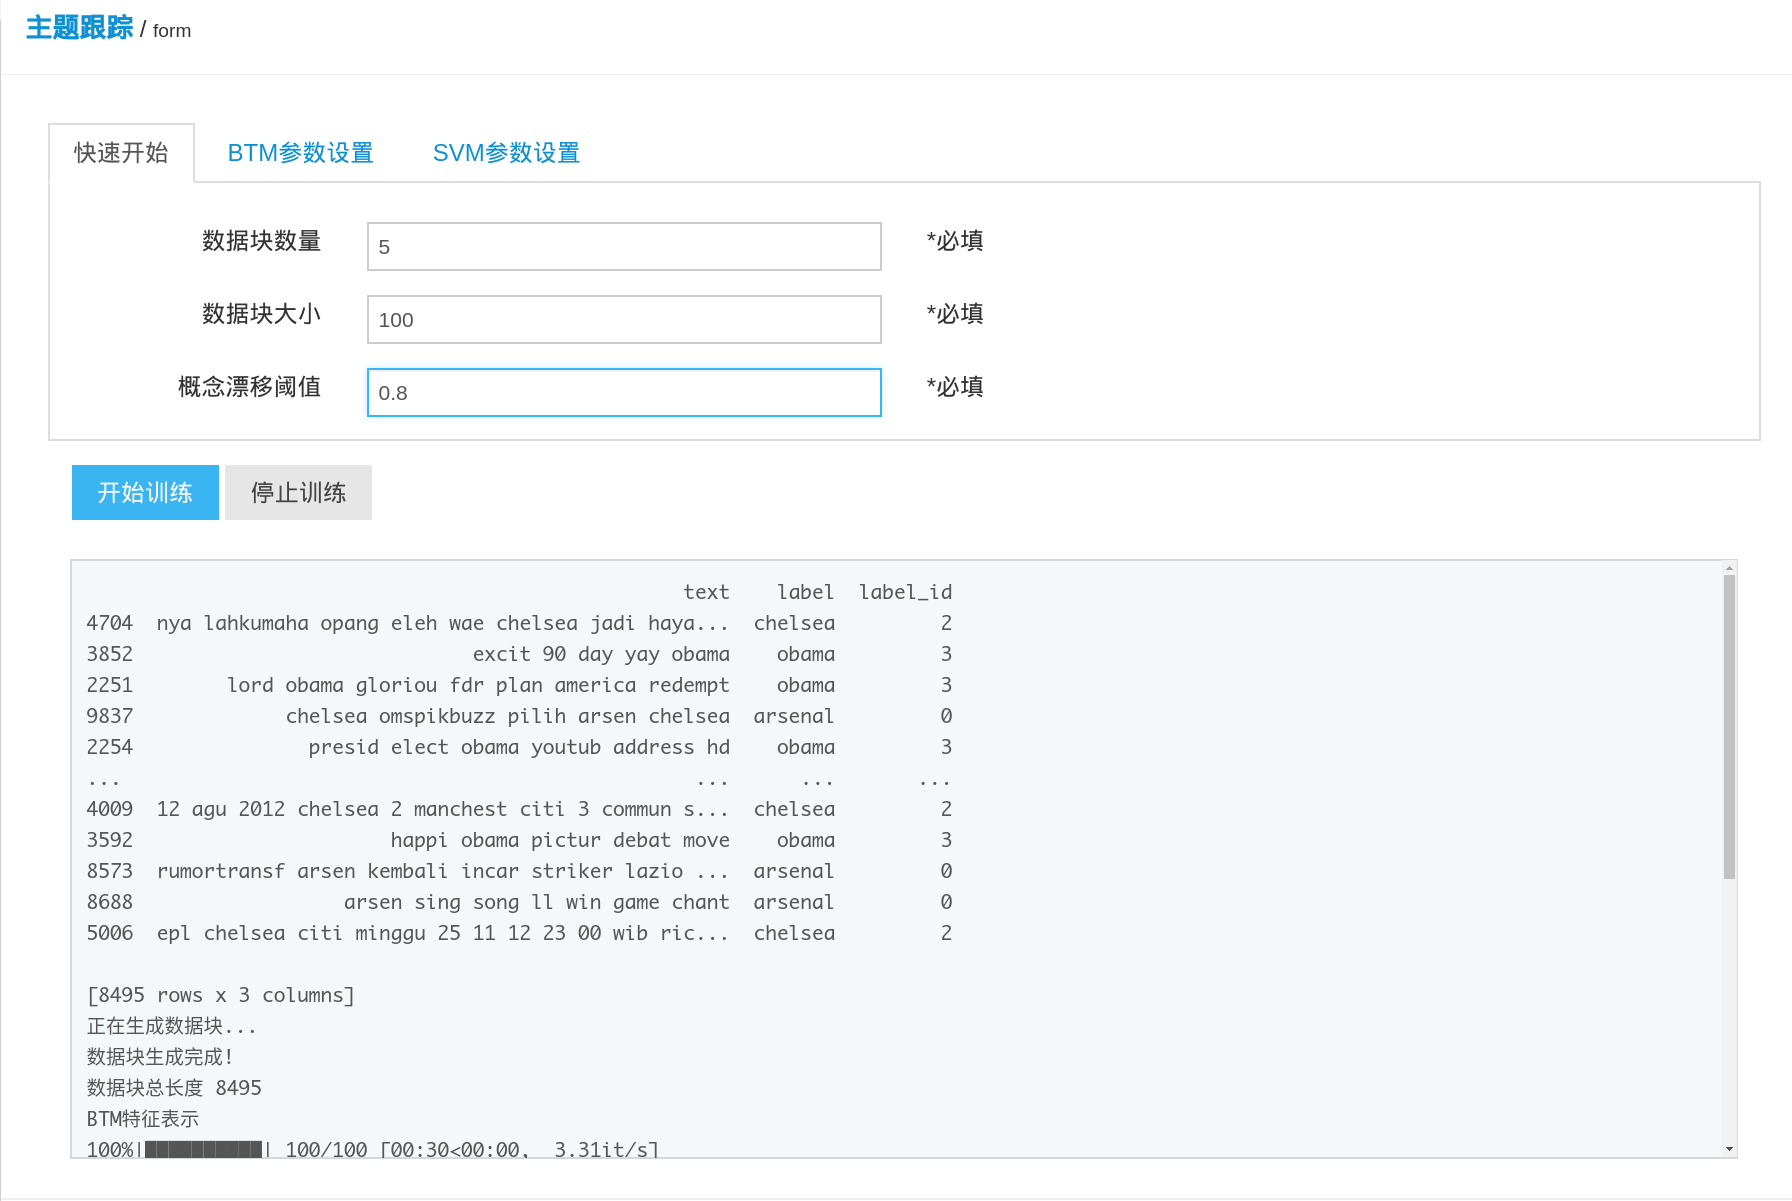
\includegraphics[width=1.0\textwidth]{topic}
  \caption{主题跟踪模块}
  \label{fig:topic}
\end{figure}

用户设置好参数后,点击“开始训练”,前端即发起请求,后端URL将请求进行分发,调用
topicProcess()函数进行主题跟踪,该函数会将数据库中的数据读出,放入一个Pandas的dataframe对象
中并打乱,用于模拟数据流,接着数据流被分块传入集成模型中进行训练,动态更新集成模型。前端通过Websocket建立长连接,
实时将训练日志输出到前端页面中,并展示主题的追踪结果。

该模块的URL路由:
\begin{minted}{py}
urlpatterns = [
    re_path('^$', topic),
    re_path('topicProcess', topicProcess)
]
\end{minted}

主题跟踪模块视图函数:
\begin{minted}{py}
@csrf_exempt
def topicProcess(request):
    try:
        if request.method == 'POST':
            # 获取前端传入参数
            H = int(request.POST['H'])
            blocksize = int(request.POST['blocksize'])
            u = float(request.POST['u'])
            ... ...
            # 获取数据流
            for label in labels_:
                query = DataModel.objects.filter(label=label)
                for row in query:
                    texts.append(row.text)
                    labels.append(row.label)
            ... ...
            data.dropna(axis=0, how='any', inplace=True)
            data = shuffle(data)
            # 初始化集成模型
            E = Ensemble(H = H, blocksize = blocksize, u = u,
            base = "svm", K = K, btm_iterations = iter,
            svm_gamma = "auto", svm_C = C, svm_kernel = "linear")
            # 集成模型训练              
            E.fit(data.text, data.label_id)
            ... ...
    except Exception as e:
        print(e)
\end{minted}

% 为了更加方便地对数据流进行操作,使用Python面向对象编程,将数据流抽象成为了数据块类Block,
% 并使用迭代器实现了对数据块的实时生成。

% 做好上述的准备工作后,即可将对带有类标签数据通过Block的形式传入集成学习模型中进行模型训练与更新,最后得到一组大小为H的基分类器集,使用得到的模型即可完成对未知标签数据进行预测和主题分析。

% 下面是整个算法的测试代码(考虑篇幅,已简化部分代码):
% \begin{minted}{py}
%     from sklearn.model_selection import train_test_split
%     from sklearn import preprocessing
%     from sklearn.feature_extraction.text import TfidfVectorizer

%     # 通过ORM模型从数据库读出数据,保存到textDF数据结构中;
%     query = DataModel.objects.all()
%     textDF = pandas.DataFrame()
    
%     ......

%     # 分割数据集,并提取TF-IDF值;
%     X_train, X_test, y_train, y_test = train_test_split(textDF.text, textDF.label, test_size=0.25, random_state=23)
%     vec_tfidf = TfidfVectorizer()
%     vec_tfidf_f = vec_tfidf.fit(X_train)
%     train_dtm_ngram = vec_tfidf_f.transform(X_train).toarray()
%     test_dtm_ngram = vec_tfidf_f.transform(X_test).toarray()
    
%     # 对标签进行向量化编码;
%     encoder = preprocessing.LabelEncoder()
%     y_train = encoder.fit_transform(y_train)
%     y_test = encoder.fit_transform(y_test)
    
%     # 使用Ensemble进行分类测试;
%     E = Ensemble(H=10, blocksize=100)
%     a = train_dtm_ngram[0]

%     # 对数据流生成数据块,并通过定义生成器生成测试数据;
%     f = E.gen_blocks(test_dtm_ngram, y_test)
%     block = next(f)
%     test_x = block.getX()
%     test_y = block.getY()

%     # 集成模型的训练;
%     E.fit(train_dtm_ngram, y_train)
%     y_pred = E.predict(test_x)
    
%     from sklearn import metrics
%     from sklearn.metrics import classification_report

%     # 分类评价指标;
%     recall = metrics.recall_score(test_y, y_pred)
%     F1 = metrics.f1_score(test_y, y_pred)
%     print("正确率:", np.mean(y_pred == test_y))
%     print("召回率:", recall)
%     print("F1:", F1)

%     # 打印评价报告;
%     target_names = ['obama', 'smartphone']
%     print(classification_report(test_y, y_pred, target_names=target_names))
    
% \end{minted}

\subsection{数据可视化模块}
该模块主要用于图表的展示,使用Echart模块进行图表绘制,其中包括对源数据中的文本进行词频统计,
分别统计数据集中每个类簇的文本总数,生成条形图和饼状图。统计每个文档的长度,使用折线图表示
各长度文档出现的频率,可以很清楚的发现,长度在40左右的文档最多,这符合社交网络中文本的特征。使用主题模型分析文本数据,通过设置主题数,对文本进行主题划分,得到主题分布图。

\begin{figure}[H]
  \centering
  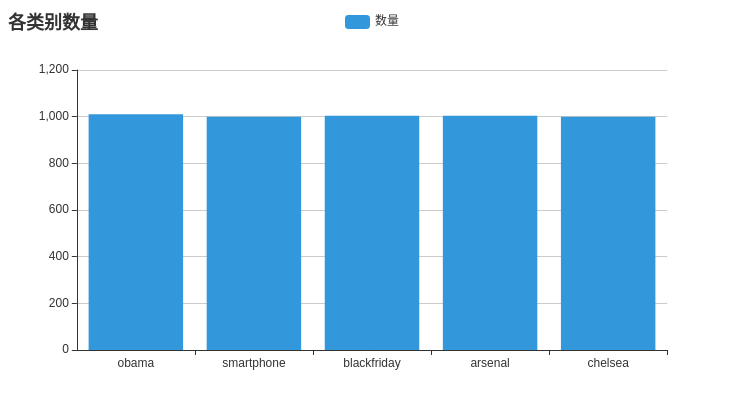
\includegraphics[width=1.0\textwidth]{fig1}
  \caption{各类别数量图}
  \label{fig:upload}
\end{figure}

\begin{figure}[H]
  \centering
  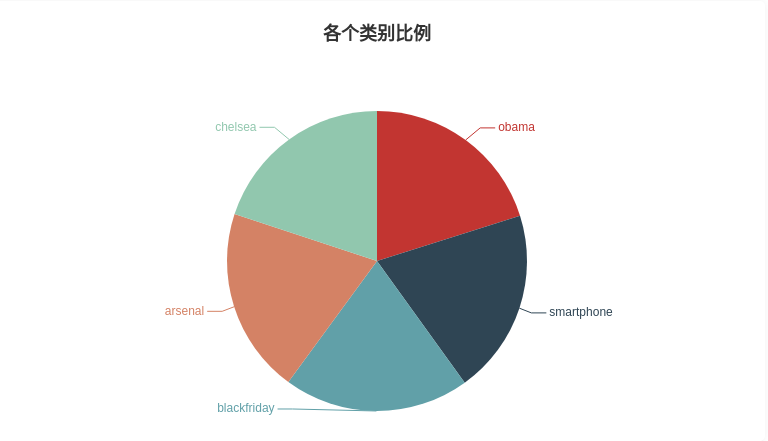
\includegraphics[width=1.0\textwidth]{fig2}
  \caption{各类别比例图}
  \label{fig:upload}
\end{figure}

\begin{figure}[H]
  \centering
  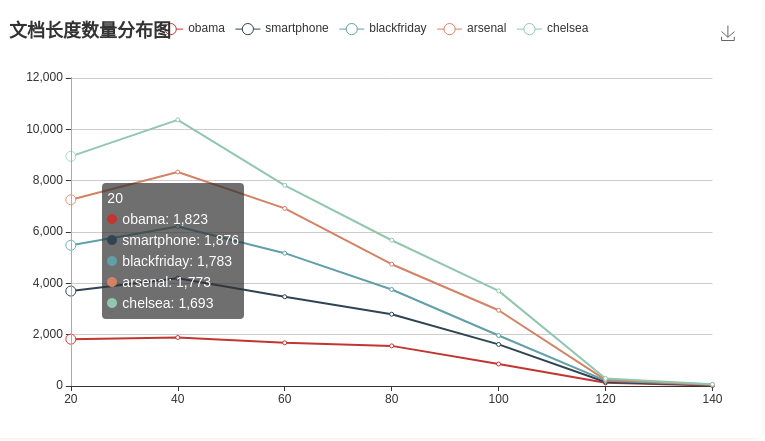
\includegraphics[width=1.0\textwidth]{fig3}
  \caption{文档长度数量分布图}
  \label{fig:upload}
\end{figure}

% \subsection{应用案例}

\section{本章小结}
本章主要介绍了Twitter数据挖掘可视化平台的搭建,使用的技术包括但不限于Django开发框架、
Scikit-learn、pandas、numpy、echart、mongodb等。以Django框架为Web平台主体,使用Scikit-learn
进行算法实现,完成了整个平台的技术整合。实现的功能模块包括:数据上传、数据预处理、数据可视
化、主题跟踪等。将数据挖掘中需要使用到的如数据预处理与数据清洗、特
征提取、分
类算法应用等过程UI化,大大降低了使用者的门槛。同时,也使研究人员能及时、快速发现研究中的问
题,具有较高的应用价值。


